\documentclass[11pt,a4paper]{article}
\usepackage[utf8]{inputenc}
\usepackage[T1]{fontenc}
\usepackage{lmodern}
\renewcommand{\abstractname}{Resumen}
\renewcommand{\contentsname}{Índice}
\renewcommand{\figurename}{Figura}
\renewcommand{\tablename}{Tabla}
\renewcommand{\refname}{Referencias}
\renewcommand{\appendixname}{Anexo}
\emergencystretch=3em
\usepackage[margin=2.4cm]{geometry}
\usepackage{microtype}
\usepackage{booktabs,longtable,array,tabularx}
\usepackage{colortbl}
\usepackage{xcolor}
\usepackage{graphicx}
\usepackage{float}
\usepackage{enumitem}
\usepackage{fancyhdr}
\usepackage{titlesec}
\usepackage[most]{tcolorbox}
\usepackage[hidelinks]{hyperref}

\definecolor{azul}{HTML}{1F4E79}
\definecolor{gris}{HTML}{F2F2F2}
\definecolor{azulclaro}{HTML}{DCE6F1}
\definecolor{naranja}{HTML}{C55A11}
\definecolor{naranjaclaro}{HTML}{FBE9DC}
\definecolor{verde}{HTML}{2E7D32}
\definecolor{verdeclaro}{HTML}{E6F2E7}
\titleformat{\section}{\Large\bfseries\color{azul}}{\thesection}{0.6em}{}
\titleformat{\subsection}{\large\bfseries\color{azul}}{\thesubsection}{0.6em}{}
\titleformat{\subsubsection}{\normalsize\bfseries}{\thesubsubsection}{0.6em}{}
\setlist{itemsep=2pt,topsep=4pt}
\setlength{\parskip}{4pt}
\setlength{\parindent}{0pt}
\renewcommand{\arraystretch}{1.2}
\pagestyle{fancy}\fancyhf{}
\fancyhead[L]{\small El junior de IA hoy y lo que muestran las carreras}
\fancyhead[R]{\small Fundamentos de Ciencia de Datos · UNSTA}
\fancyfoot[C]{\small\thepage}
\renewcommand{\headrulewidth}{0.3pt}

\newtcolorbox{caja}[1][]{colback=gris,colframe=azul,boxrule=0.6pt,arc=2pt,left=8pt,right=8pt,top=6pt,bottom=6pt,#1}
\newtcolorbox{resultado}[1][]{enhanced,colback=verdeclaro,colframe=verde,boxrule=0.6pt,arc=2pt,left=10pt,right=8pt,top=6pt,bottom=6pt,borderline west={3pt}{0pt}{verde},title={},#1}
\newtcolorbox{decision}[1][]{enhanced,colback=naranjaclaro,colframe=naranja,boxrule=0.6pt,arc=2pt,left=10pt,right=8pt,top=6pt,bottom=6pt,borderline west={3pt}{0pt}{naranja},#1}
\newtcolorbox{enunasola}[1][]{enhanced,colback=azulclaro,colframe=azul,boxrule=0pt,arc=2pt,left=8pt,right=8pt,top=4pt,bottom=4pt,#1}
\newcommand{\NA}{\textsc{na}}
\setlength{\aboverulesep}{0pt}\setlength{\belowrulesep}{0pt}
\renewcommand{\le}{\ensuremath{\leq}}
\renewcommand{\ge}{\ensuremath{\geq}}
\newcolumntype{L}[1]{>{\raggedright\arraybackslash}p{#1}}
\newcolumntype{C}[1]{>{\centering\arraybackslash}p{#1}}

\begin{document}

% ---------------- PORTADA ----------------
\begin{tcolorbox}[enhanced,colback=azul,colframe=azul,arc=3pt,left=14pt,right=14pt,top=12pt,bottom=12pt]
{\small\color{white}Universidad del Norte Santo Tomás de Aquino · Ingeniería en Inteligencia Artificial · Tucumán, Argentina\\Fundamentos de Ciencia de Datos · 3.\textsuperscript{er} año · Observatorio de IA, edición 1 (corte 06/11/2026)}\par
\vspace{0.4cm}
{\fontsize{24}{28}\selectfont\bfseries\color{white} El junior de IA hoy y lo que muestran las carreras}\par
\vspace{0.2cm}
{\large\color{white} Qué habilidades piden los avisos de nivel de entrada en roles de IA y cuánto de eso aparece en lo que publican las carreras argentinas de IA}
\end{tcolorbox}
\vspace{0.3cm}
{\large Matías Alejandro Chalín · Lucio Agustín Sappia · Luciano Aquiles Tartarini}\par
{\normalsize Docente: Rodrigo Zottola · Tucumán, noviembre de 2026}\par
\vspace{0.3cm}

\begin{abstract}\noindent
Estudiamos si las prácticas de producción de la IA (integración, despliegue, monitoreo, nube y contenedores, y control de versiones) tienen menos evidencia publicada en los planes de estudio de carreras argentinas de IA que las habilidades de base (Python, SQL, estadística, aprendizaje automático clásico y aprendizaje profundo), aunque los avisos de nivel de entrada también las piden. Capturamos 18.206 avisos únicos de nueve fuentes el 06/11/2026, seleccionamos los de nivel de entrada de roles de IA con reglas escritas antes de mirar habilidades y obtuvimos una muestra de 97 avisos de 61 empresas. Con una línea de base automática, el 76\,\% de los avisos de entrada de la muestra menciona al menos una práctica de producción y el 62\,\% al menos una habilidad de base. Codificamos con cita textual las cinco carreras que publican contenidos por materia (cuatro instituciones): la evidencia publicada de base fue en promedio 55 puntos porcentuales mayor que la de producción ($\Delta = 0{,}55$; intervalo de confianza del 95\,\%: 0,30 a 0,80). Las cuatro instituciones van en el mismo sentido y el resultado se mantiene al cambiar los casos límite, pero cuatro instituciones son pocas y la lectura humana de los avisos y la segunda lectura de los planes siguen pendientes. Las otras seis carreras publican solo títulos o folletos y no pueden evidenciar prácticas de producción; se declaran como límite y no se usan en el análisis principal. El informe fija el método completo, con cada decisión justificada, para que cualquier persona pueda repetirlo.
\end{abstract}

\tableofcontents
\bigskip

\section*{Lectura rápida (para quien lee primero)}
\begin{caja}
\textbf{Qué preguntamos.} Si alguien busca su primer trabajo en IA, ¿qué le piden los avisos y cuánto de eso muestran los planes de las carreras argentinas de IA?\par
\textbf{Qué hicimos.} Juntamos 18.206 avisos de empleo, nos quedamos con los de nivel de entrada de roles de IA (97 avisos, 61 empresas) y leímos con cita textual los planes de cinco carreras que publican el contenido de cada materia.\par
\textbf{Qué encontramos.} (1) Solo 12\,\% de los avisos de IA es de nivel de entrada. (2) Esos avisos piden a menudo prácticas de producción: despliegue (60\,\%), nube y contenedores (40\,\%), integración (34\,\%). (3) Los planes muestran mucho más las habilidades de base que las de producción: la diferencia promedio es de 55 puntos porcentuales (intervalo 30 a 80), y va en el mismo sentido en las cuatro instituciones.\par
\textbf{Cómo confiar en esto.} Confianza media: son pocas instituciones, los avisos se marcaron con un diccionario automático y la lectura humana sigue pendiente (sección \ref{sec:confianza}). Publicar menos no es enseñar menos.\par
\textbf{Qué no es.} No es un ranking, no mide calidad de enseñanza ni empleo, y no vale para el mercado argentino en general.
\end{caja}

\begin{figure}[H]
\centering
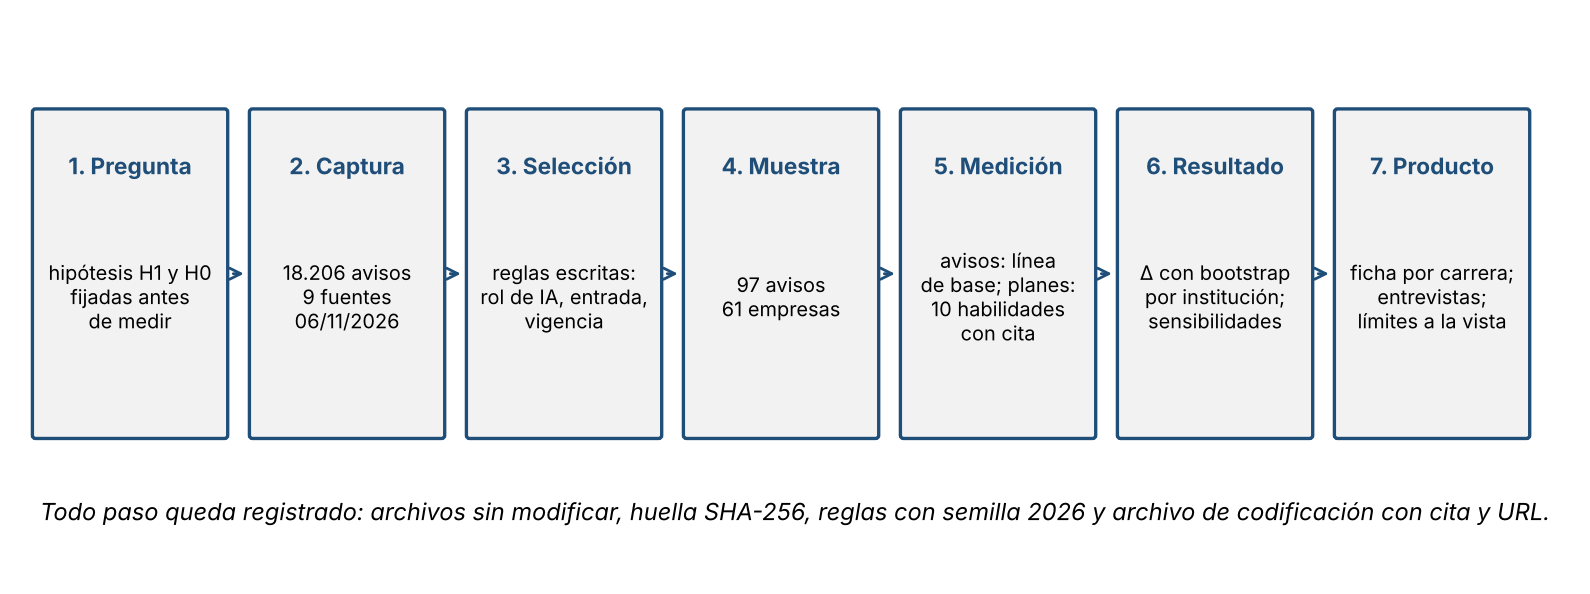
\includegraphics[width=\textwidth]{fig_flujo.png}
\caption{Recorrido completo del trabajo, de la pregunta al producto. Cada paso se detalla en las secciones 2 a 7.}
\end{figure}

% ---------------- 1 ----------------
\section{Problema, pregunta e hipótesis}

\begin{caja}
\textbf{Qué hacemos y para qué.} Medimos qué habilidades piden hoy los avisos de nivel de entrada en roles de IA y las comparamos con lo que publican los planes de estudio de once carreras argentinas. El resultado sirve para que una dirección de carrera vea, con fuentes y límites a la vista, qué habilidades de producción están poco documentadas en su plan. No mide empleo, calidad de la enseñanza ni aprendizaje.
\end{caja}

\subsection{Por qué importa}
Un plan de estudios se diseña con años de anticipación y los puestos de entrada cambian más rápido. En los sistemas de aprendizaje automático el modelo suele ser una parte pequeña del sistema, y llevarlo a producción y mantenerlo genera trabajo propio \cite{sculley2015,paleyes2022}. Si los avisos de entrada piden esas tareas y los planes no las muestran, conviene saberlo con datos. Si los avisos de entrada de IA son pocos, eso también es un hallazgo.

\subsection{Conceptos que usamos}
\begin{itemize}
\item \textbf{Aviso de nivel de entrada.} Aviso cuyo texto pide como máximo 2 años de experiencia (sección \ref{sec:reglas}). No usamos la etiqueta de nivel de las plataformas porque probamos que no es confiable.
\item \textbf{Rol de IA.} Aviso cuyo título nombra un rol de IA o ciencia de datos.
\item \textbf{Habilidades de base:} Python, SQL, estadística, aprendizaje automático clásico y aprendizaje profundo.
\item \textbf{Habilidades de producción:} integración (conectar un modelo con otras aplicaciones, por ejemplo mediante una API), despliegue (ponerlo en el entorno donde se usa de verdad), monitoreo (controlar mientras se usa si sigue funcionando bien), nube y contenedores, y control de versiones (Git).
\item \textbf{IA actual:} modelos de lenguaje, recuperación aumentada y uso de APIs de modelos. Solo se describe; no entra en la hipótesis.
\item \textbf{Evidencia publicada.} Una celda carrera--habilidad vale 1 si el plan publicado muestra la habilidad y \NA{} (información insuficiente) si no. \NA{} nunca se cuenta como ``cero'' en el informe: que algo no se vea no prueba que no se enseñe.
\end{itemize}

\subsection{Pregunta e hipótesis}
\textbf{Pregunta.} ¿Qué habilidades y tareas piden hoy los avisos de nivel de entrada en roles de IA y cuánto de eso aparece en lo que publican las carreras argentinas de IA?

\textbf{H1.} En los planes publicados, las habilidades de producción tienen menos evidencia que las de base, aunque los avisos de nivel de entrada también piden las de producción.

\textbf{H0.} La evidencia publicada de producción no es menor que la de base.

\textbf{Cómo se decide.} Para cada carrera se calcula la proporción de habilidades de base con evidencia y la de producción con evidencia. La diferencia $\Delta$ es la media de la primera menos la media de la segunda. El intervalo de confianza del 95\,\% de $\Delta$ se obtiene por remuestreo (\emph{bootstrap}) de instituciones, con 10.000 remuestreos y semilla 2026. H1 queda \emph{sostenida} si el límite inferior es mayor que 0, \emph{refutada} si el límite superior es menor que 0 y \emph{sin resolver} en cualquier otro caso. Se informa la magnitud de $\Delta$ y no se inventa un umbral de ``diferencia relevante''.

\textbf{Qué parte decide cada fuente.} La diferencia entre base y producción se decide con las carreras. Los avisos solo sostienen la segunda parte (``aunque los avisos también las piden'') y se describen aparte.

\subsection{Alcance}
Entra: avisos de nivel de entrada en roles de IA y planes publicados de once carreras. Queda fuera: salarios, calidad de la enseñanza, empleo real, rankings de universidades o de empresas y datos personales.

\subsection{Antecedentes y fuentes de referencia}\label{sec:antecedentes}
Estas fuentes dan contexto y justifican decisiones de diseño. No son datos del estudio y no trasladamos sus porcentajes a nuestros resultados. En la búsqueda que hicimos no encontramos un estudio que compare, para Argentina y para el nivel de entrada, lo que piden los avisos con lo que publican los planes de las carreras de IA; por eso el aporte es acotado y lo presentamos como un relevamiento y no como una evaluación de las carreras.

\begin{table}[H]
\centering\small
\begin{tabularx}{\textwidth}{L{3.1cm} X X}
\toprule
\rowcolor{azulclaro}\textbf{Fuente} & \textbf{Qué respalda} & \textbf{Su límite para este estudio}\\
\midrule
Sculley et al. (2015) \cite{sculley2015} & En los sistemas de aprendizaje automático el modelo es una parte pequeña y el resto (datos, integración, mantenimiento) genera deuda técnica. Justifica que las prácticas de producción merezcan medirse aparte & Es un argumento de ingeniería, no mide qué piden los avisos ni qué enseñan las carreras\\
Paleyes, Urma y Lawrence (2022) \cite{paleyes2022} & Revisión de casos reales de despliegue: las dificultades aparecen en cada etapa, también después de entrenar el modelo. Respalda tratar despliegue y monitoreo como habilidades propias & Reúne casos publicados, sin distinguir puestos de entrada\\
Shankar et al. (2022) \cite{shankar2022} & Entrevistas a 18 ingenieros de aprendizaje automático: el éxito en producción depende de velocidad, validación y versionado. Respalda incluir el control de versiones entre las prácticas de producción & Muestra pequeña y de ingenieros con experiencia; no son puestos de entrada\\
Lanubile, Martínez-Fernández y Quaranta (2023) \cite{lanubile2023} & Una asignatura universitaria puede enseñar el ciclo completo de un componente de aprendizaje automático, con despliegue y monitoreo, mediante proyectos. Muestra que estas prácticas son enseñables en un curso de grado & Es un caso de dos universidades europeas con una evaluación preliminar; no describe la oferta argentina\\
Azuara y Jaramillo (2026) \cite{azuara2026} & Nota técnica del BID que analiza más de 6,2 millones de vacantes digitales de 15 países de América Latina entre 2022 y 2025, con habilidades digitales y de IA. Respalda usar avisos en línea como indicador de demanda & Los avisos en línea cubren solo una parte de la demanda laboral. No se centra en el nivel de entrada de roles de IA ni compara con planes\\
Brown, Cai y DasGupta (2001) \cite{brown2001} & Márgenes de error de una proporción: fundamento de los mínimos de 30 y 100 avisos & Es un método estadístico, no una fuente sobre el tema\\
Efron (1979) \cite{efron1979} & Remuestreo (\emph{bootstrap}) para intervalos de confianza sin suponer una distribución & Con pocos grupos (aquí cuatro instituciones) el intervalo es aproximado\\
Landis y Koch (1977) \cite{landis1977} & Interpretación del coeficiente kappa; fundamento del piso de 0,6 & Sus rangos son una convención ampliamente usada, no una regla\\
Strathern (1997) \cite{strathern1997} & Cuando una medida se vuelve meta deja de ser una buena medida; fundamento de no publicar rankings & Es un argumento general, no un resultado empírico sobre carreras de IA\\
\bottomrule
\end{tabularx}
\caption{Fuentes de referencia, qué respalda cada una y su límite.}
\end{table}

% ---------------- 2 ----------------
\section{Datos}
\begin{enunasola}\textbf{En una frase.} de dónde salen los avisos y los planes, con qué reglas se eligen y qué sesgos tiene cada fuente.\end{enunasola}


\subsection{Fuentes y método de obtención}
Los métodos se declaran tal como se ejecutaron. La lectura y codificación posterior de cada aviso es manual; la captura de los avisos fue automatizada.

\begin{table}[H]
\centering\small
\begin{tabularx}{\textwidth}{L{3.2cm} L{4.6cm} r X}
\toprule
\rowcolor{azulclaro}\textbf{Fuente} & \textbf{Método} & \textbf{Avisos únicos} & \textbf{Observación}\\
\midrule
LinkedIn Argentina & Scraping automatizado (Apify, actor \texttt{dataji/apify-linkdin-jobs} v0.0.7), 06/11/2026, 15:11--15:17 & 279 & 648 filas brutas; aprobado por el Directorio; ver sección \ref{sec:legal}\\
Greenhouse & API pública de tableros & 11.264 & Tableros descubiertos en hilos de HN\\
Ashby & API pública de tableros & 4.487 & Idem\\
Lever & API pública de tableros & 1.549 & Idem\\
Himalayas & API pública & 223 & Agregador de trabajo remoto\\
Jobicy & API pública & 133 & La consulta en español dio error 400\\
RemoteOK & API pública & 99 & Agregador de trabajo remoto\\
Remotive & API pública & 12 & La API devuelve pocos avisos\\
Get on Board & API pública & 160 & Texto solo para lectura humana\\
\midrule
\textbf{Total} & & \textbf{18.206} & 9 fuentes\\
\bottomrule
\end{tabularx}
\caption{Fuentes, método y avisos únicos capturados.}
\end{table}

\textbf{LinkedIn.} Se usó el actor de Apify ``LinkedIn Jobs Scraper'', que no requiere iniciar sesión y devuelve la descripción completa. Parámetros: ubicación Argentina; sin filtro de nivel de LinkedIn; exclusión de títulos con \emph{senior, sr, lead, principal, staff, head, manager, director}; descripción completa; tope de 300 por búsqueda. Cuatro búsquedas: \emph{machine learning}, \emph{AI engineer}, \emph{data scientist} e \emph{inteligencia artificial}, que cubren los nombres más comunes del puesto en inglés y en español (decisión del equipo, no validada contra otras palabras). Resultado: 648 filas brutas y 279 avisos únicos por identificador, porque el mismo aviso aparecía en varias búsquedas. Costo: unos USD 0,60. Dos pruebas se descartaron: el filtro de nivel ``Entry level'' de LinkedIn (100 avisos, casi todos \emph{Senior} o \emph{Lead}) y el filtro por títulos con \emph{junior, jr, entry, trainee, associate, intern} (0 avisos).

\textbf{Tableros de empresas.} Los enlaces a Greenhouse, Lever y Ashby se extrajeron de 36 hilos mensuales ``Ask HN: Who is hiring?'' con la API pública de Algolia. Se descubrieron 513 tableros; 411 respondieron y 102 ya no existen (error 404 o 410). \textbf{Sesgo declarado:} solo entran empresas que publicaron en esos hilos, en su mayoría de tecnología y de habla inglesa. Por eso los resultados globales no representan el mercado argentino y se analizan por grupo de acceso.

\textbf{Buenas prácticas de captura.} Nos identificamos con un \emph{User-Agent} (``UNSTA-student-project, academic research''); hay pausas de 1 s entre pedidos (2 s en agregadores); cada respuesta se guarda sin modificar, con fecha UTC y huella SHA-256 en un manifiesto; no se recolectan datos personales y no se evaden restricciones.

\subsection{Aspectos legales y éticos}\label{sec:legal}
\begin{itemize}
\item \textbf{LinkedIn.} Sus términos restringen la captura automatizada. El Directorio del Observatorio aprobó este método de captura para fines académicos. Por eso se declara como scraping automatizado y no como manual. Los textos de los avisos no se redistribuyen: se publican resultados agregados y los identificadores.
\item \textbf{Get on Board.} Su \texttt{robots.txt} declara \texttt{ai-train=no}. Por eso su texto no se procesa de forma automática: se codifica solo a mano. Del procesamiento automático solo se usa su campo estructurado de nivel (\emph{seniority}).
\item \textbf{Resto de las fuentes.} Son APIs públicas documentadas, usadas solo para investigación académica.
\item \textbf{Planes de estudio.} Son páginas y PDF públicos; se citan y no se redistribuyen.
\end{itemize}

\subsection{Reglas de selección}\label{sec:reglas}
Las reglas se fijaron antes de mirar habilidades y se aplican igual a todas las fuentes. Así ningún aviso se elige por lo que menciona.

\begin{table}[H]
\centering\small
\begin{tabularx}{\textwidth}{L{2.7cm} L{4.6cm} L{2.2cm} X}
\toprule
\rowcolor{azulclaro}\textbf{Regla} & \textbf{Definición} & \textbf{Tipo} & \textbf{Justificación}\\
\midrule
Rol de IA & El título contiene términos como \emph{AI, ML, LLM, NLP, machine learning, data scientist, deep learning, inteligencia artificial, computer vision, generative, agentic} & Decisión del equipo & Es verificable y repetible. Limitación: se pierden roles con títulos genéricos; se estima con una muestra de control\\
Trabaja con modelos & Lectura humana: el puesto implica entrenar, evaluar, integrar o desplegar modelos & Decisión del equipo & El título solo no alcanza (``AI Sales Manager'' no es un rol técnico)\\
Nivel de entrada & Máximo de años de experiencia mencionado en contexto de experiencia \le{} 2; se ignoran números mayores a 20 & Convención y decisión & Se mide por lo que el aviso exige. Se usa el máximo y no el mínimo para que ``1 a 5 años'' no entre. Sensibilidad: \le{}1, \le{}3 y Entry+Associate\\
Contexto de experiencia & El número cuenta si cerca (80 caracteres) aparecen palabras como \emph{experiencia, trabajo, background} & Decisión del equipo & Evita contar ``empresa fundada hace 15 años''. Sensibilidad: ventanas de 40 y 120\\
Get on Board & Entrada si su nivel declarado es \emph{No experience required} o \emph{Junior} & Convención & Es un campo estructurado; no hace falta leer el texto\\
Sin dato de años & Se resuelven por lectura humana & Decisión del equipo & No se asume ni entrada ni no entrada\\
Vigencia & Publicado hace 365 días o menos & Decisión del equipo & La pregunta es sobre ``hoy''; un año cubre un ciclo de contratación. Con 180 días quedan 156 avisos y con 730, 166 (antes de limpiar)\\
Texto suficiente & 100 palabras o más & Decisión del equipo & Con menos texto no se distingue lo que el aviso pide\\
Duplicados & Mismo identificador cuenta como uno; entre avisos de entrada, mismo \texttt{empresa + título} cuenta como uno & Decisión del equipo & Una vacante en varias ciudades no es evidencia nueva\\
Tope por empresa & Máximo 10 avisos por empresa, elegidos con semilla 2026 & Decisión del equipo & Equivale al 10\,\% de la meta de 100 avisos. Sin tope, dos empresas ocuparían 59 de 166 avisos (36\,\%). Se reporta también sin tope\\
Grupo de acceso & Argentina; LatAm o mundial declarado; remoto sin país; otra región & Decisión del equipo & Separa lo que alcanza un egresado argentino del resto\\
\bottomrule
\end{tabularx}
\caption{Reglas de selección, tipo de justificación y sensibilidad.}
\end{table}

\subsection{Embudo de población}
\begin{table}[H]
\centering\small
\begin{tabular}{L{9.2cm} r}
\toprule
\rowcolor{azulclaro}\textbf{Paso} & \textbf{Avisos}\\
\midrule
Avisos únicos capturados (9 fuentes) & 18.206\\
Rol de IA por título & 1.413\\
\quad con nivel de entrada (\le{}2 años o declarado) & 166\\
\quad con nivel sin dato (a resolver por lectura humana) & 496\\
Entrada y rol de IA, vigentes (\le{}365 días) & 163\\
\quad con texto de 100 palabras o más & 161\\
\quad sin repetir empresa y título & 104\\
\quad con tope de 10 por empresa: \textbf{muestra de análisis} & \textbf{97}\\
\bottomrule
\end{tabular}
\caption{Del total capturado a la muestra de análisis.}
\end{table}

\begin{figure}[H]
\centering
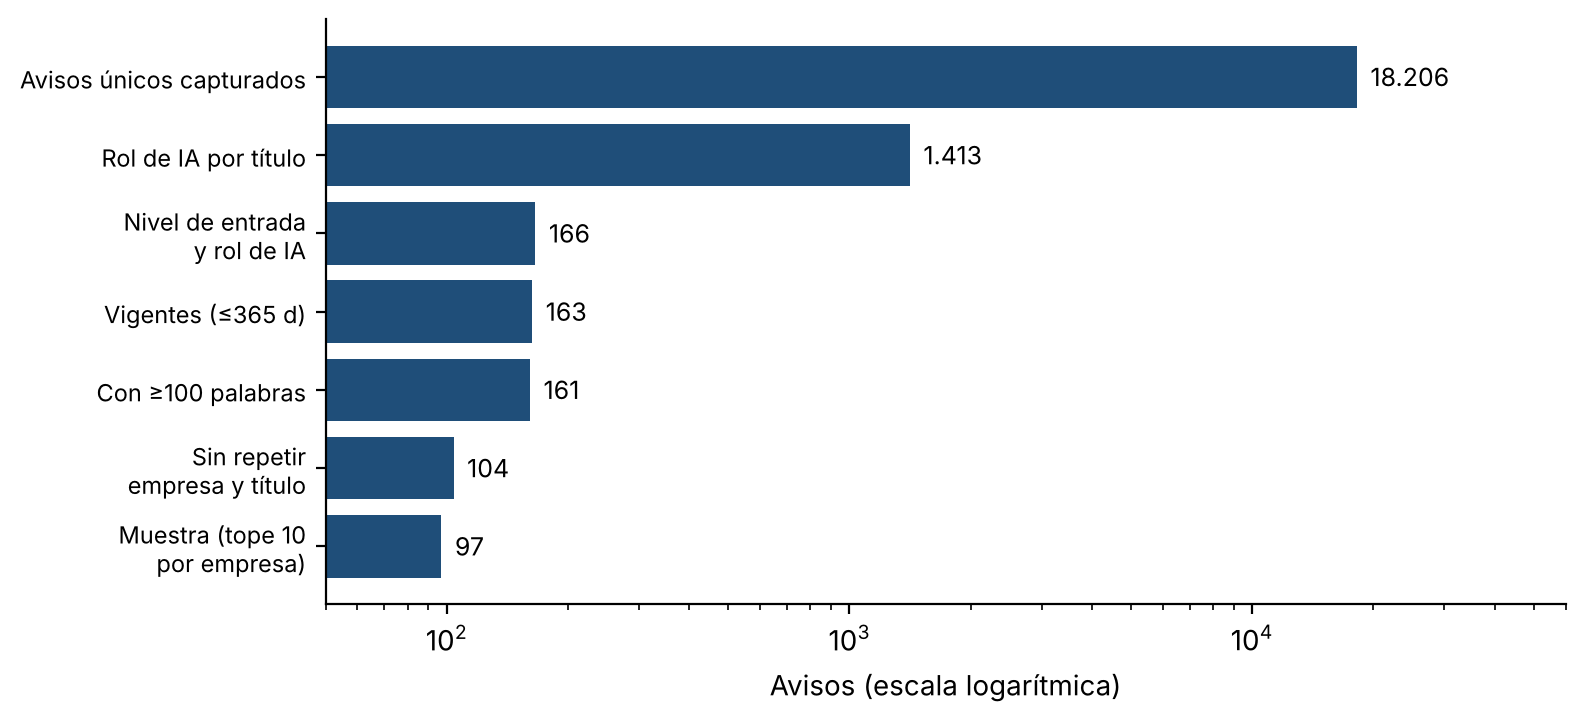
\includegraphics[width=0.85\textwidth]{fig_embudo.png}
\caption{Embudo de selección (escala logarítmica). La mayor caída es el paso a nivel de entrada: de 1.413 avisos de IA quedan 166.}
\end{figure}

Solo el 12\,\% de los avisos de IA (166 de 1.413) es de nivel de entrada. Es un resultado en sí mismo.

\subsection{La muestra de análisis}
\begin{itemize}
\item \textbf{Tamaño:} 97 avisos de 61 empresas, con un máximo de 10 por empresa.
\item \textbf{Fuente:} Greenhouse 42, Ashby 24, Himalayas 13, LinkedIn 12, Lever 3, Get on Board 2 y Jobicy 1.
\item \textbf{Acceso:} 81 de otra región, 15 de Argentina (12 empresas) y 1 remoto sin país.
\item \textbf{Idioma:} 85 en inglés y 12 en español, todos de LinkedIn. El libro de códigos cubre ambos idiomas.
\item \textbf{Longitud:} mediana de 633 palabras (mínimo 104, máximo 1.878). Fechas entre 11/2025 y 11/2026.
\item \textbf{Años pedidos:} 4 avisos piden 0 años, 23 piden 1 y 68 piden 2; los otros 2 son de Get on Board y se clasifican por su campo declarado.
\end{itemize}

\textbf{Suficiencia.} Se necesitan al menos 30 avisos para reportar un porcentaje (convención). Con 30 avisos y un porcentaje del 50\,\%, el margen de error del 95\,\% es de unos $\pm$18 puntos; con 100, de unos $\pm$10 \cite{brown2001}. La muestra de 97 alcanza el mínimo y queda apenas por debajo de la meta de 100. Dos grupos no alcanzan el mínimo y solo se describen: los 15 avisos de Argentina y los 27 avisos que piden 1 año o menos.

\subsection{Calidad de los datos y transformaciones}
Antes de medir se buscaron errores, faltantes, duplicados y sesgos. Cada transformación se hizo en un script y no se modificó ningún archivo crudo.

\begin{table}[H]
\centering\small
\begin{tabularx}{\textwidth}{L{3.2cm} L{4.4cm} X}
\toprule
\textbf{Problema} & \textbf{Qué se encontró} & \textbf{Qué se hizo}\\
\midrule
Duplicados & LinkedIn: 648 filas brutas para 279 avisos (el mismo aviso salía en varias búsquedas). Entre avisos de entrada, 161 pasan a 104 al unir empresa y título repetidos & Se deja uno por identificador y uno por empresa y título; se informa cuántos se eliminan\\
Años de experiencia faltantes & 5.329 avisos de la población total, y 496 de rol de IA, no mencionan años & Se clasifican ``sin dato'' (ni entrada ni no entrada) y se resuelven por lectura humana; no se asume nada\\
Años atípicos & Números como ``fundada hace 25 años'' o mayores a 20 & Se ignoran los mayores a 20 y solo cuentan los que están cerca de palabras de experiencia\\
Fechas & Himalayas y Get on Board venían en segundos y se leían como milisegundos (año 1970) & Corregido; el cambio de huella quedó registrado (anexo B)\\
Texto muy corto & 2 avisos vigentes de entrada y rol de IA tenían menos de 100 palabras & Se excluyen (regla D9)\\
Tableros inexistentes & 102 de 513 tableros ya no existen (404 o 410) & Se registran como inexistentes; no son error del proceso\\
Cobertura de Argentina & Solo 15 de 97 avisos & Se describe aparte y no se generaliza\\
Idioma & 85 en inglés y 12 en español & El diccionario cubre ambos; el límite se declara\\
Sesgo de fuente & Los tableros salen de empresas que publicaron en hilos de HN & Se declara y se analiza por grupo de acceso\\
\bottomrule
\end{tabularx}
\caption{Controles de calidad, hallazgos y tratamiento.}
\end{table}

\subsection{Los planes de las once carreras}
El universo son once carreras de diez instituciones (Palermo tiene dos títulos), las que el equipo pudo documentar entre el 07 y el 14/10/2026. Es un universo, no una muestra, y no se hacen pruebas de hipótesis sobre él. El nivel documental indica cuánto publica cada carrera: \emph{identificación} (un tríptico), \emph{listado} (títulos de materias) o \emph{contenidos} (contenidos por materia).

\begin{table}[H]
\centering\small
\begin{tabular}{L{7.0cm} L{2.6cm} L{3.4cm}}
\toprule
\rowcolor{azulclaro}\textbf{Carrera} & \textbf{Institución} & \textbf{Nivel documental}\\
\midrule
Licenciatura en Inteligencia Artificial y Ciencia de Datos & UADE & contenidos\\
Ingeniería en Inteligencia Artificial & Palermo & contenidos\\
Licenciatura en Inteligencia Artificial & Palermo & contenidos\\
Ingeniería en Inteligencia Artificial & UNL & contenidos\\
Licenciatura en Inteligencia Artificial (plan 2026, Ord. 2188) & UTN-FRLP & contenidos\\
Ingeniería en Inteligencia Artificial & UNSTA & listado\\
Carrera de IA & UCA & listado\\
Carrera de IA & UdeSA & listado\\
Carrera de IA & Siglo 21 & listado\\
Carrera de IA & UCC & listado\\
Carrera de IA & UCEMA & identificación\\
\bottomrule
\end{tabular}
\caption{Las once carreras y su nivel documental. Los nombres exactos de las seis carreras con listado o identificación se completan al cargar su ficha.}
\end{table}

\textbf{Protocolo.} Se consulta el sitio oficial de cada institución. Para las cinco carreras con contenidos, el 06/11/2026 releímos directamente la página oficial del plan (UADE, Palermo, UNL) o el PDF de la ordenanza (UTN-FRLP) y registramos, para cada celda positiva, la asignatura, la cita textual y la URL (archivo \texttt{codificacion\_planes.csv}). No guardamos copia con huella SHA-256 de esas páginas, así que quien repita el trabajo debe guardar su propia copia fechada y anotar si el plan cambió. La obtención es manual porque los sitios son pocos y heterogéneos (HTML, PDF, tríptico) y automatizarla no aportaría valor.

\begin{caja}
\textbf{Riesgo principal: sesgo por nivel documental.} Una carrera que publica solo títulos deja ver ``Programación'' o ``Estadística'', pero casi nunca ``despliegue'' o ``monitoreo'', que aparecen en los contenidos. La evidencia de producción saldría más baja por falta de detalle documental y no por falta de formación. Para evitarlo, el análisis principal de H1 usa solo las cinco carreras de nivel \emph{contenidos} (cuatro instituciones) y las once carreras (diez instituciones) quedan como sensibilidad. La unidad de remuestreo es la institución porque las dos carreras de Palermo no son independientes. Con cuatro instituciones el intervalo será ancho; si incluye el 0, el resultado es ``sin resolver'' y es un resultado válido.
\end{caja}

% ---------------- 3 ----------------
\section{Método de medición}
\begin{enunasola}\textbf{En una frase.} qué cuenta como cada habilidad, cómo se mide y por qué se eligieron cada umbral y cada método.\end{enunasola}


\subsection{Libro de códigos}
Cada habilidad se codifica 1 si el texto muestra que se pide (aviso) o se enseña (plan), y 0 en un aviso si no aparece. En un plan, la ausencia de evidencia es \NA{}. Cuenta la mención de la tarea o la herramienta como parte del trabajo; no cuenta como pedida si solo aparece en la descripción de la empresa.

\begin{table}[H]
\centering\small
\begin{tabularx}{\textwidth}{L{2.4cm} L{2.4cm} X}
\toprule
\rowcolor{azulclaro}\textbf{Grupo} & \textbf{Habilidad} & \textbf{Cuenta cuando el texto\ldots}\\
\midrule
Base & Python & nombra Python\\
Base & SQL & nombra SQL o una base de datos relacional\\
Base & Estadística & nombra estadística, probabilidad o pruebas de hipótesis\\
Base & ML clásico & nombra técnicas o bibliotecas concretas (scikit-learn, árboles, bosques aleatorios, regresiones, \emph{clustering}); ``machine learning'' a secas no alcanza\\
Base & Aprendizaje profundo & nombra redes neuronales, \emph{deep learning}, PyTorch, TensorFlow o Keras\\
Producción & Integración & pide construir o usar APIs, servicios o microservicios que conectan el modelo con otras aplicaciones\\
Producción & Despliegue & pide llevar o tener modelos en producción (\emph{deploy}, CI/CD, \emph{serving})\\
Producción & Monitoreo & pide monitorear modelos o sistemas en uso (\emph{drift}, observabilidad); ``mantener'' a secas no alcanza\\
Producción & Nube y contenedores & nombra AWS, Azure, GCP, Docker, Kubernetes o similares\\
Producción & Git & nombra Git, GitHub, GitLab o control de versiones\\
IA actual & LLM, RAG, APIs de modelos & nombra modelos de lenguaje, RAG, agentes, \emph{prompts} o APIs de proveedores de modelos (solo descriptivo)\\
\bottomrule
\end{tabularx}
\caption{Habilidades codificadas. La lista de palabras de la línea de base figura en el anexo A.}
\end{table}

\subsection{Línea de base y lectura humana}
\textbf{Línea de base.} Un diccionario de palabras y expresiones en español e inglés, fijado antes de ver resultados, marca cada habilidad en cada aviso. Es rápido, repetible y burdo: puede marcar una habilidad que el aviso solo nombra de pasada y puede perder expresiones que no previmos. Por eso es una línea de base y no una medida final.

\textbf{Lectura humana.} Los 97 avisos de la muestra se leen dos veces, de forma independiente, por dos integrantes del equipo con asignación rotativa y semilla registrada (con 97 avisos es viable leerlos todos, así que no hace falta una submuestra). Se mide el acuerdo con el coeficiente kappa de Cohen y se exige un valor de 0,6 o más, el piso de lo que Landis y Koch llaman acuerdo sustancial \cite{landis1977}. Cada desacuerdo se resuelve por escrito y queda registrado.

\textbf{Por qué no entrenamos un clasificador.} Con 97 avisos no hay datos para entrenar y validar un modelo sin engañarnos. La línea de base validada por lectura humana es suficiente. Si la población crece a cientos de avisos, un clasificador podrá compararse contra esta línea de base.

\textbf{Planes.} Se leen los planes con el mismo libro de códigos y cada celda positiva lleva una cita textual con su fuente y fecha de consulta. Regla de decisión para los casos límite: una habilidad cuenta si el texto la \emph{nombra} (por ejemplo, ``SQL o ``Python) o nombra una tarea que el libro de códigos define; una alusión genérica (``versionado, ``lenguajes de acceso a bases de datos relacionales) no cuenta, y cada caso límite se informa y se prueba en la sensibilidad. Esta regla es estricta y puede subestimar tanto la base como la producción.

\subsection{Cálculos}
\begin{itemize}
\item \textbf{Demanda.} Porcentaje de avisos que piden cada habilidad, con intervalo del 95\,\%. Los avisos de una misma empresa no son independientes, así que se remuestrean empresas completas \cite{efron1979}.
\item \textbf{Cobertura y $\Delta$.} Como se describió en la sección 1.3, con remuestreo de instituciones.
\item \textbf{Sensibilidades.} Se repite el cálculo cambiando una decisión por vez y se compara con el resultado principal: \le{}1 y \le{}3 años; Entry+Associate; ventanas de contexto de 40 y 120 caracteres; vigencia de 180 y 730 días; sin tope por empresa; sin Get on Board; solo Argentina (descriptivo). En los planes: cambiar cada caso límite de codificación y comparar las cinco carreras de contenidos con las once (esto último queda pendiente, ver sección \ref{sec:estado}). Si el veredicto cambia en alguna, se declara frágil.
\end{itemize}

\subsection{Decisiones estadísticas y su justificación}
\begin{table}[H]
\centering\small
\begin{tabularx}{\textwidth}{L{3.3cm} L{2.6cm} L{2.2cm} X}
\toprule
\rowcolor{azulclaro}\textbf{Decisión} & \textbf{Valor} & \textbf{Tipo} & \textbf{Por qué}\\
\midrule
Nivel de confianza & 95\,\% & Convención & Es el valor habitual en la práctica estadística\\
Remuestreos & 10.000 & Convención & Estabiliza los extremos del intervalo; con menos, cambian de una corrida a otra\\
Semilla & 2026 & Convención & Hace repetible el resultado; el valor concreto es irrelevante\\
Unidad de remuestreo & Empresa (avisos); institución (planes) & Decisión del equipo & Los avisos de una empresa y las carreras de una institución no son independientes\\
Mínimo para un porcentaje & 30 avisos & Convención & Margen de unos $\pm$18 puntos; menos sería ruido\\
Meta de población & 100 avisos & Decisión del equipo & Margen de unos $\pm$10 puntos\\
Acuerdo entre lectores & kappa $\geq$ 0,6 & Estándar & Acuerdo sustancial según \cite{landis1977}\\
Años de entrada & \le{} 2 & Convención & Es lo que suele entenderse por puesto inicial; la sensibilidad muestra cuánto depende\\
Diferencia relevante & Ninguna fijada & Decisión del equipo & No hay base para inventarla; se informa la magnitud y el intervalo\\
Entrevistas & 3 a 5 & Decisión del equipo & Mínimo para ver coincidencias entre más de dos personas y máximo que podemos coordinar y analizar en el plazo\\
\bottomrule
\end{tabularx}
\caption{Umbrales estadísticos.}
\end{table}

% ---------------- 4 ----------------
\section{Resultados disponibles}
\begin{enunasola}\textbf{En una frase.} qué piden los avisos de entrada, qué muestran los planes y qué dice H1; todo con su nivel de confianza.\end{enunasola}

Esta sección informa solo lo que ya está medido. Los resultados que dependen de la lectura humana y de la codificación de los planes figuran como pendientes en la sección \ref{sec:estado}.

\subsection{Demanda de habilidades en los avisos de entrada (línea de base)}
Se aplicó el diccionario a los 95 avisos de la muestra cuyo texto puede procesarse automáticamente (se excluyen los 2 de Get on Board) y a las 59 empresas que los publican.

\begin{figure}[H]
\centering
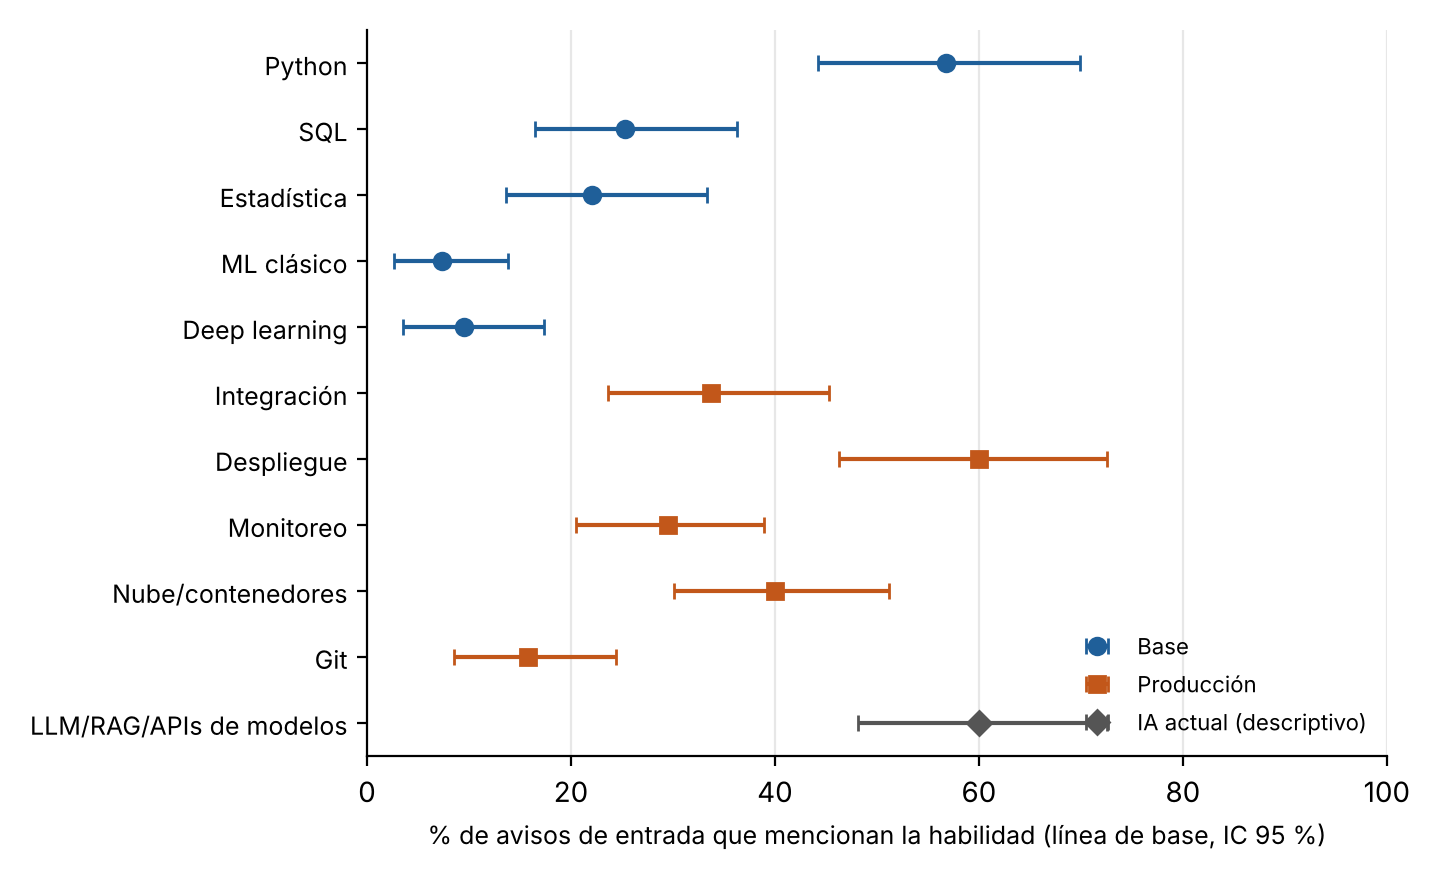
\includegraphics[width=0.92\textwidth]{fig_demanda.png}
\caption{Porcentaje de avisos de entrada que mencionan cada habilidad, con intervalo del 95\,\% por remuestreo de empresas. Línea de base automática, sin validar por lectura humana.}
\end{figure}

\begin{table}[H]
\centering\small
\begin{tabular}{L{4.4cm} L{2.6cm} r r l}
\toprule
\rowcolor{azulclaro}\textbf{Habilidad} & \textbf{Grupo} & \textbf{Avisos} & \textbf{\%} & \textbf{IC 95\,\%}\\
\midrule
Python & Base & 54 & 56,8 & 44,2--69,9\\
SQL & Base & 24 & 25,3 & 16,5--36,3\\
Estadística & Base & 21 & 22,1 & 13,6--33,3\\
ML clásico & Base & 7 & 7,4 & 2,6--13,8\\
Aprendizaje profundo & Base & 9 & 9,5 & 3,5--17,4\\
Integración & Producción & 32 & 33,7 & 23,6--45,3\\
Despliegue & Producción & 57 & 60,0 & 46,3--72,6\\
Monitoreo & Producción & 28 & 29,5 & 20,5--38,9\\
Nube y contenedores & Producción & 38 & 40,0 & 30,1--51,2\\
Git & Producción & 15 & 15,8 & 8,5--24,4\\
LLM, RAG, APIs de modelos & IA actual & 57 & 60,0 & 48,1--72,6\\
\midrule
Al menos una de base & Resumen & 59 & 62,1 & 50,0--74,7\\
Al menos una de producción & Resumen & 72 & 75,8 & 63,4--86,5\\
Integración, despliegue y monitoreo a la vez & Resumen & 15 & 15,8 & 9,0--24,1\\
\bottomrule
\end{tabular}
\caption{Demanda por habilidad en 95 avisos de entrada de 59 empresas (línea de base automática).}
\end{table}

\textbf{Lectura.} Los avisos de entrada de la muestra piden con frecuencia prácticas de producción: despliegue en 60\,\%, nube y contenedores en 40\,\%, integración en 34\,\% y monitoreo en 30\,\%; Git es la menos mencionada (16\,\%). Esto respalda la parte ``aunque los avisos de entrada también las piden''. Al menos una práctica de producción aparece en el 76\,\% de los avisos, frente al 62\,\% de al menos una de base, pero los intervalos se superponen y no corresponde afirmar una diferencia entre esos dos porcentajes. Python (57\,\%) es la habilidad de base más pedida. ML clásico y aprendizaje profundo salen bajos porque el diccionario exige nombrar técnicas o herramientas concretas.

\textbf{Dos precauciones.} (1) Es una línea de base: ``despliegue'' puede marcarse cuando el aviso solo dice ``en producción'' de forma genérica y la lectura humana puede corregirlo. (2) Solo 15 avisos son de Argentina; en ellos, 11 mencionan alguna práctica de producción y 10 alguna de base. Son conteos descriptivos que no permiten generalizar. Con el criterio de 1 año o menos (27 avisos, por debajo del mínimo de 30) el patrón es parecido: 52\,\% menciona alguna de base y 52\,\% alguna de producción, solo a modo descriptivo.

\subsection{Evidencia publicada en las carreras con contenidos}\label{sec:planes}
Codificamos las diez habilidades en las cinco carreras de nivel \emph{contenidos}, con el libro de códigos de la sección 3.1 y la regla de la sección 3.2. Cada celda positiva tiene asignatura, cita textual y URL en el archivo de codificación; la figura muestra el resultado.

\begin{figure}[H]
\centering
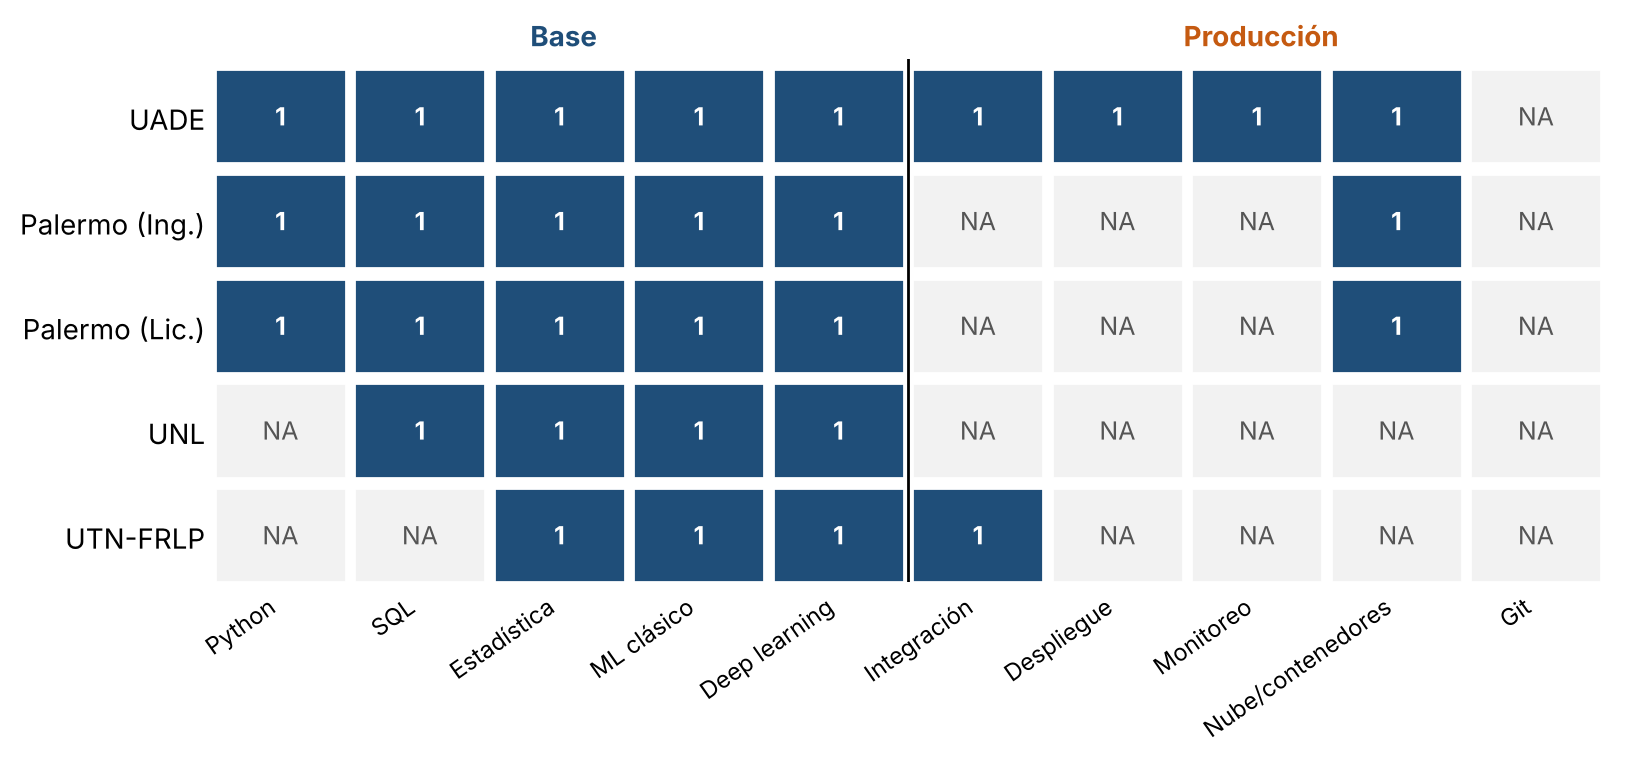
\includegraphics[width=\textwidth]{fig_planes.png}
\caption{Evidencia publicada por carrera: 1 = el plan muestra la habilidad (con cita), NA = información insuficiente (no es ``cero''). Carreras con evidencia, de 5: Python 3, SQL 4, estadística 5, ML clásico 5, aprendizaje profundo 5, integración 2, despliegue 1, monitoreo 1, nube y contenedores 3, Git 0.}
\end{figure}

La proporción de habilidades con evidencia por carrera, de base y de producción, es: UADE 1,0 y 0,8; Palermo (ambos títulos) 1,0 y 0,2; UNL 0,8 y 0,0; UTN-FRLP 0,6 y 0,2. La diferencia $\Delta$ de cada carrera es la resta: 0,2; 0,8; 0,8; 0,8 y 0,4.

\textbf{Qué muestran las citas.} La evidencia de despliegue y monitoreo está solo en UADE (``Seminario integrador de ciencia de datos'': ``Implementación y despliegue de modelos en un entorno de producción'' y ``Monitoreo y mantenimiento de modelos en producción''), que también nombra servicios de nube (``Canalización e integración de servicios de nube'': AWS SageMaker, Google AI Platform, Azure Machine Learning). En Palermo la nube aparece como tema en ``Big Data'' (``Cloud. IoT'') y en ``Procesamiento de Lenguaje Natural'' (``Servicios para procesamiento intensivo en la nube''), no como práctica de despliegue. La integración en UTN-FRLP está en el objetivo de ``Visión Artificial y Lenguaje Natural'' (Ordenanza 2188, p.~36): ``Desarrollar aplicaciones que integren modelos de PLN y visión por computadora''. Ninguna de las cinco carreras nombra Git.

\textbf{Casos límite, decididos antes de calcular.}
\begin{itemize}
\item \emph{UADE, integración:} se codificó 1 por ``Integración de tecnologías de inteligencia artificial en flujos de trabajo empresariales'' (Automatización de procesos empresariales con AI). Es una alusión cercana pero no a APIs; se prueba en la sensibilidad.
\item \emph{UNL, Git:} ``Versionado'' (Laboratorio de Datos II) no nombra Git ni control de versiones; se codificó \NA{}.
\item \emph{UTN-FRLP, Python y SQL:} el plan nombra scikit-learn, pandas y matplotlib (Aprendizaje Automático, p.~33) y ``Lenguajes de acceso a Bases de Datos Relacionales'' (p.~28), pero no ``Python'' ni ``SQL''; se codificó \NA{}.
\item \emph{UTN-FRLP, monitoreo:} ``Monitoreo y gestión de redes'' es monitoreo de redes de computadoras, no de modelos; no cuenta.
\item \emph{UNL, Python:} el plan nombra ``Programación I a III'' sin decir el lenguaje; \NA{}.
\end{itemize}

\subsection{Resultado de H1}
Cada institución aporta un valor de $\Delta$ (Palermo promedia sus dos títulos): UADE 0,2; Palermo 0,8; UNL 0,8; UTN-FRLP 0,4. El promedio es $\Delta = 0{,}55$ (55 puntos porcentuales) con intervalo del 95\,\% de 0,30 a 0,80, por remuestreo de las cuatro instituciones (10.000 remuestreos, semilla 2026). Como el límite inferior es mayor que 0, según la regla fijada en la sección 1.3, H1 queda sostenida en este conjunto.

\begin{resultado}
\textbf{Resultado.} En las cinco carreras que publican contenidos, la evidencia publicada de base supera a la de producción en 0,55 en promedio (intervalo del 95\,\%: 0,30 a 0,80). \textbf{H1 queda sostenida en este conjunto}, con confianza media: son cuatro instituciones y un solo lector en los planes.
\end{resultado}

\begin{figure}[H]
\centering
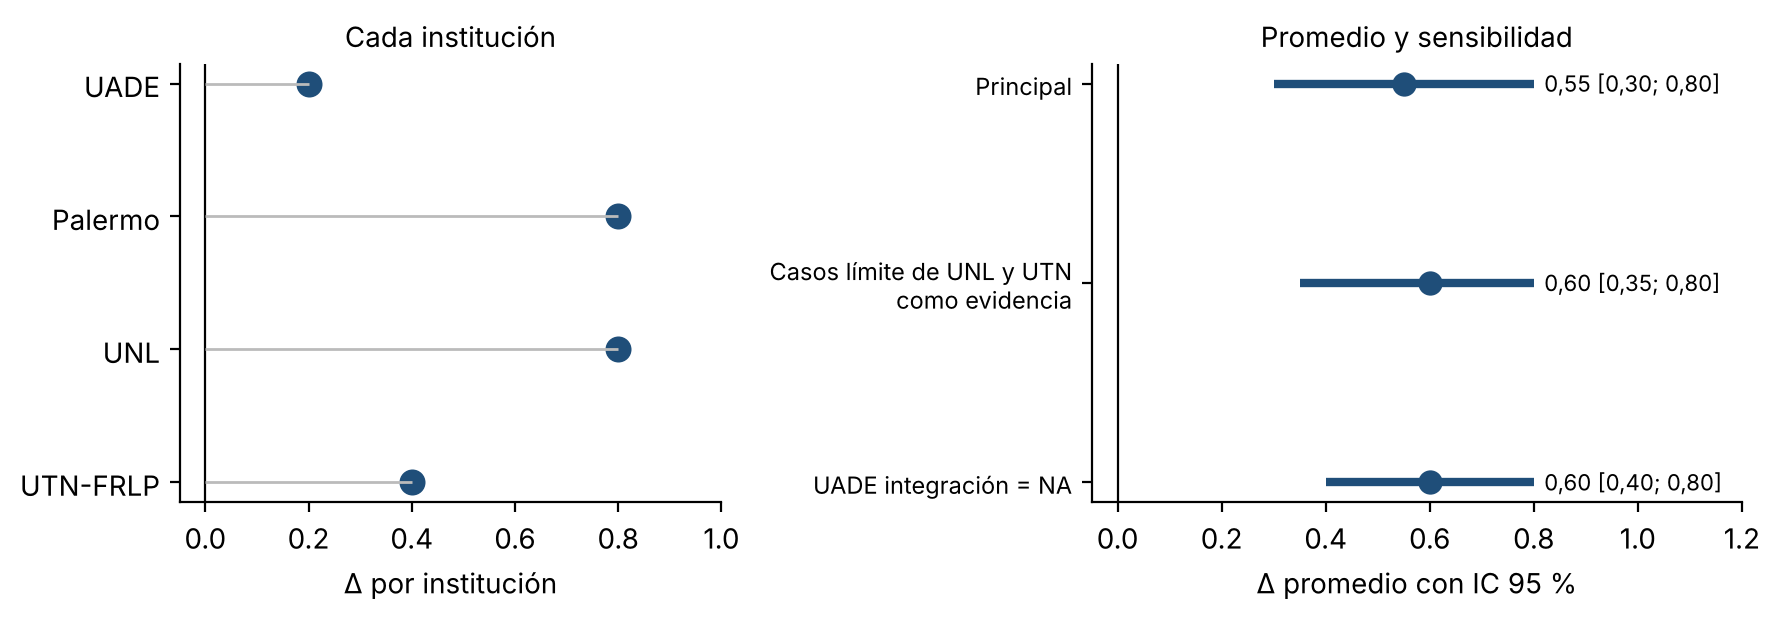
\includegraphics[width=0.95\textwidth]{fig_delta.png}
\caption{$\Delta$ por institución (izquierda) y promedio con intervalo del 95\,\% en el escenario principal y en dos escenarios de sensibilidad (derecha). La línea vertical en 0 es ``sin diferencia''.}
\end{figure}

\begin{table}[H]
\centering\small
\begin{tabular}{L{8.4cm} c l}
\toprule
\rowcolor{azulclaro}\textbf{Escenario} & \textbf{$\Delta$} & \textbf{IC 95\,\%}\\
\midrule
Principal (codificación estricta) & 0,55 & 0,30--0,80\\
Los tres casos límite de UNL y UTN-FRLP codificados como evidencia & 0,60 & 0,35--0,80\\
UADE integración como \NA{} & 0,60 & 0,40--0,80\\
\bottomrule
\end{tabular}
\caption{Sensibilidad del resultado a los casos límite.}
\end{table}

\textbf{Cómo leer el resultado de H1, sin exagerar.}
\begin{enumerate}
\item El sentido es el mismo en las cuatro instituciones ($\Delta > 0$ en todas) y en los tres escenarios; el veredicto no cambia.
\item Con solo cuatro instituciones, si las cuatro tienen $\Delta > 0$ el límite inferior queda por encima de 0 casi por construcción, y el intervalo por remuestreo es aproximado \cite{efron1979}. Una prueba de signos exacta con 4 de 4 daría $p = 0{,}0625$ (unilateral), por encima de 0,05. Por eso lo presentamos como un resultado consistente y acotado, no como una prueba fuerte.
\item Es un resultado sobre lo que las carreras \emph{publican}. No dice que lo que no se publica no se enseñe, ni compara calidad de las carreras.
\item La parte ``aunque los avisos de entrada también las piden'' se apoya en la línea de base de la sección 4.1: despliegue 60\,\%, nube y contenedores 40\,\%, integración 34\,\% y monitoreo 30\,\% de los avisos. Esa línea aún no pasó por lectura humana.
\item La codificación de los planes fue hecha por un solo lector, asistido por una herramienta de IA, con verificación de cada cita. Falta una segunda lectura independiente de los planes, con kappa.
\item Las seis carreras restantes publican solo títulos o folletos. Con títulos no se puede evidenciar ``despliegue'' o ``monitoreo'', por eso no se usan en el análisis principal (sección 2.7). Su codificación queda como sensibilidad pendiente.
\end{enumerate}

\subsection{Avisos frente a planes, habilidad por habilidad}
La figura siguiente junta las dos fuentes. Cada punto es una habilidad: el círculo muestra qué porcentaje de los avisos de entrada la pide y el cuadrado, qué porcentaje de las cinco carreras muestra evidencia. Son unidades distintas (avisos y carreras), por lo que la figura es descriptiva y no es una prueba.

\begin{figure}[H]
\centering
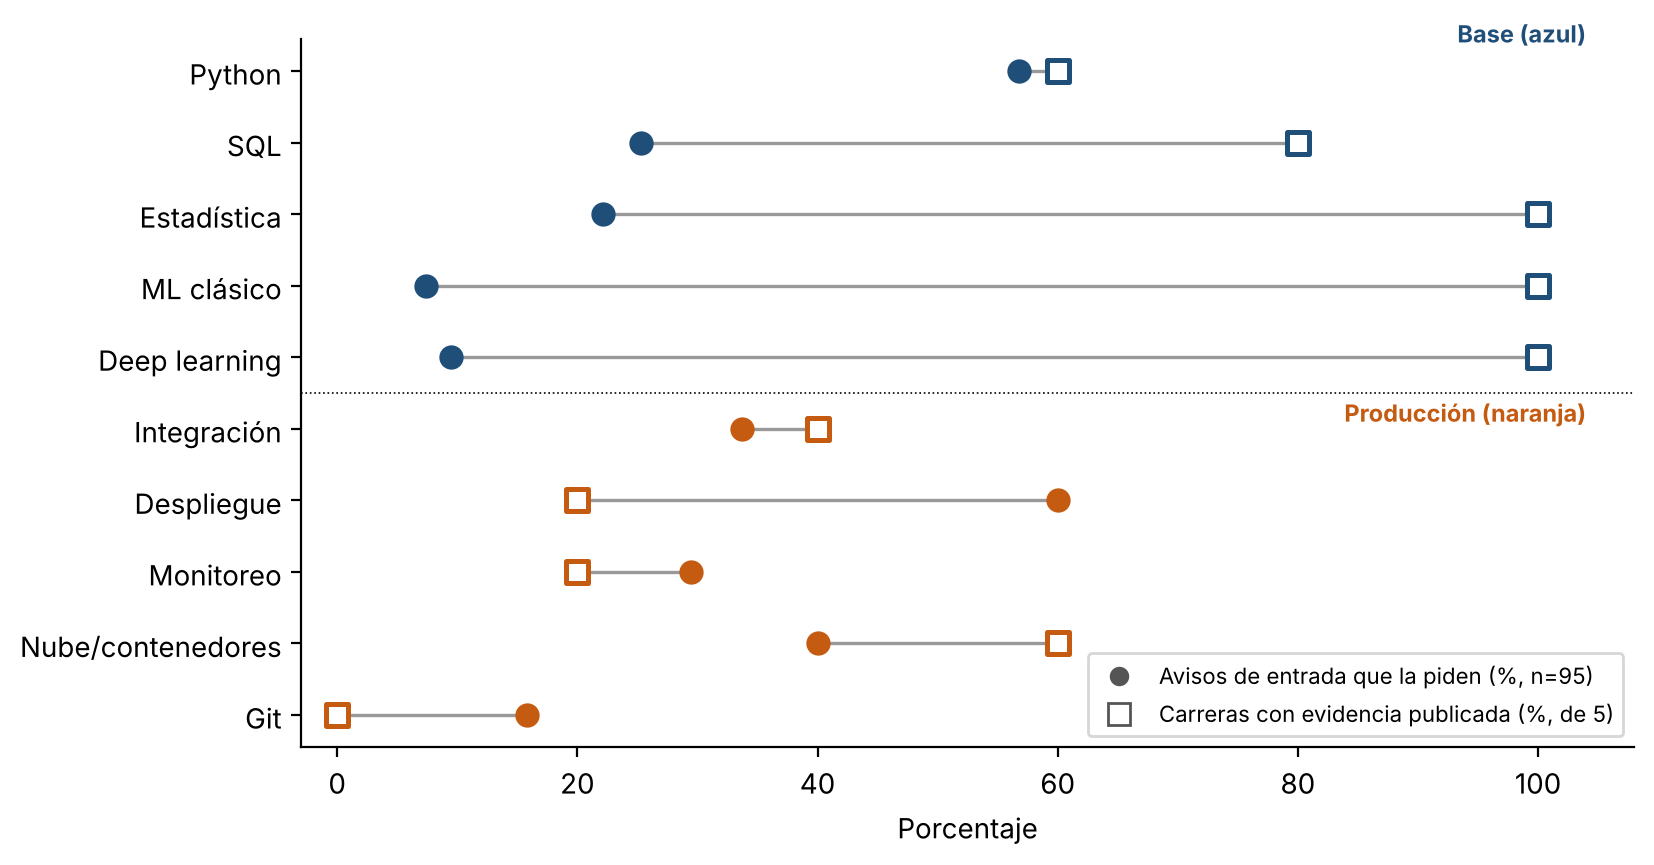
\includegraphics[width=0.92\textwidth]{fig_brecha.png}
\caption{Demanda en avisos de entrada y evidencia publicada en los planes, por habilidad.}
\end{figure}

\textbf{Lectura.} En las habilidades de base los planes están muy por encima de lo que dicen los avisos (estadística, ML clásico y aprendizaje profundo aparecen en las cinco carreras; los avisos las nombran poco porque el diccionario exige términos concretos). En producción la imagen es mixta y conviene no simplificarla: \emph{despliegue} es la habilidad con mayor distancia (60\,\% de los avisos y 1 de 5 carreras), \emph{monitoreo} y \emph{Git} también tienen poca evidencia en los planes, pero \emph{nube y contenedores} aparece en 3 de 5 carreras, más que en la proporción de avisos (40\,\%). Es decir, la brecha de producción se concentra en despliegue, monitoreo y Git.

% ---------------- 5 ----------------
\section{Validación y límites}
\begin{enunasola}\textbf{En una frase.} qué podemos afirmar, qué no, cuánto confiar en cada hallazgo y qué limita el estudio.\end{enunasola}


\begin{table}[H]
\centering\small
\begin{tabularx}{\textwidth}{L{3cm} X X}
\toprule
\rowcolor{azulclaro} & \textbf{Podemos afirmar} & \textbf{No podemos afirmar}\\
\midrule
Lo que observamos & Hay 166 avisos de entrada y de IA entre 1.413 de IA; 97 forman la muestra. Los avisos de entrada de la muestra mencionan prácticas de producción con frecuencia (línea de base). En las cinco carreras con contenidos, la evidencia publicada de base supera a la de producción en promedio por 0,55 (IC 0,30--0,80) & Que esos porcentajes sean los del mercado argentino, que la línea de base sea exacta o que el resultado valga para las seis carreras sin contenidos\\
Lo que inferimos, con prudencia & La distancia entre lo que piden los avisos de entrada y lo que publican los planes es mayor en producción que en base, en este conjunto & Que valga para toda Argentina ni para todos los planes: son cuatro instituciones\\
Lo que no afirmamos & & Que una distancia entre avisos y planes sea una carencia de la formación, o que lo que no se publica no se enseñe. Esto es una asociación entre documentos, no una relación causal\\
\bottomrule
\end{tabularx}
\caption{Qué se sostiene y qué no.}
\end{table}

\subsection{Nivel de confianza por hallazgo}\label{sec:confianza}
\begin{table}[H]
\centering\small
\begin{tabularx}{\textwidth}{L{4.6cm} L{2.0cm} X}
\toprule
\rowcolor{azulclaro}\textbf{Hallazgo} & \textbf{Confianza} & \textbf{Por qué}\\
\midrule
Solo 12\,\% de los avisos de IA capturados es de nivel de entrada & Media--alta & Conteo directo con reglas escritas; la regla de años por texto puede fallar en casos sueltos y cubre solo las fuentes capturadas\\
Los avisos de entrada piden con frecuencia prácticas de producción & Media & Línea de base automática sin lectura humana; ``despliegue'' puede marcarse por una mención genérica\\
Los planes con contenidos publican más base que producción ($\Delta = 0{,}55$) & Media & Mismo sentido en las cuatro instituciones y en las sensibilidades, pero son solo cuatro instituciones y un lector\\
La distancia se concentra en despliegue, monitoreo y Git & Media--baja & Depende de pocas carreras (despliegue y monitoreo solo en UADE) y de la regla estricta de codificación\\
Lo que pasa en Argentina & Baja & Solo 15 avisos; se describe y no se generaliza\\
Las seis carreras sin contenidos & No evaluable & Solo publican títulos o folletos\\
\bottomrule
\end{tabularx}
\caption{Nivel de confianza (criterio del equipo, justificado en la última columna).}
\end{table}

\textbf{Limitaciones principales.}
\begin{enumerate}
\item \textbf{Foto de un día.} Los avisos son los vigentes el 06/11/2026; otra fecha dará otros números.
\item \textbf{Sesgo de descubrimiento.} Los tableros salen de hilos de HN, con predominio de empresas anglosajonas. Argentina está subrepresentada (15 avisos).
\item \textbf{Rol por título.} Es repetible, pero pierde roles con títulos genéricos. Se estima con una muestra de control de 100 avisos no seleccionados.
\item \textbf{Años por texto.} La regla puede confundir años en el rol con experiencia total y no distingue ``requerido'' de ``deseable''. Se valida con la lectura humana.
\item \textbf{Idioma.} El 88\,\% de la muestra está en inglés; una diferencia entre Argentina y el resto puede mezclarse con una diferencia de idioma.
\item \textbf{LinkedIn.} Un solo país, avisos vigentes ese día y exclusión por título (senior, lead, etc.) que pudo dejar afuera algún aviso de entrada.
\item \textbf{Nivel documental.} Es el sesgo principal del lado curricular (sección 2.7) y se controla restringiendo el análisis principal.
\item \textbf{Pocas instituciones.} Son cuatro; el intervalo es aproximado y el resultado es consistente pero no concluyente (sección 4.3).
\item \textbf{Un solo lector en los planes.} La codificación la hizo una persona asistida por IA y falta segunda lectura independiente.
\item \textbf{Regla estricta.} Exigir que el plan nombre la habilidad puede subestimar la base (UTN-FRLP sin Python ni SQL) y la producción; se prueba en la sensibilidad.
\item \textbf{Conflicto de interés.} Las tres personas del equipo estudian en UNSTA, que es una de las once carreras. Su plan se codificó con las mismas reglas y no entra en el análisis principal, porque publica solo el listado de materias.
\item \textbf{Uso de herramientas de IA.} Se usó una herramienta de IA para programar, buscar y leer planes y redactar. Cada valor y cada cita se verificó contra su fuente y el equipo responde por el contenido.
\item \textbf{Fecha de publicación.} En algunas plataformas puede ser la de la última actualización.
\end{enumerate}

% ---------------- 6 ----------------
\section{Producto y validación con usuarios}
\begin{enunasola}\textbf{En una frase.} qué producto entregamos, para quién y cómo se prueba que sirve.\end{enunasola}

\textbf{Producto.} Una ficha por carrera, pensada para directores y coordinadores. Muestra el nivel documental, las diez habilidades (1 o \NA{}) con la cita y fecha de cada celda positiva, y la frecuencia con que los avisos de entrada piden cada habilidad. No es un ranking de universidades ni de empresas.

\textbf{Validación con usuarios.} Se harán entre 3 y 5 entrevistas breves a coordinadores de carrera y estudiantes, con cinco preguntas: qué entendieron al leer la ficha por primera vez; qué decisión tomarían con ella; qué falta; qué les parece engañoso o injusto; y si la volverían a usar. Se registran las respuestas y los cambios hechos en consecuencia.

\textbf{Regla de decisión sobre el valor.} Si en las entrevistas menos de la mitad entiende la ficha sin ayuda o nadie dice que tomaría una decisión con ella, se revisa el alcance y el formato antes de seguir (criterio del equipo: la utilidad se valida antes de construir más y no solo al final). Cada cambio hecho por feedback se registra en la tabla siguiente.

\begin{table}[H]
\centering\small
\begin{tabular}{L{1.3cm} L{2.4cm} L{3.6cm} L{3.6cm} L{3.4cm}}
\toprule
\textbf{Persona} & \textbf{Rol} & \textbf{Qué entendió y qué falta} & \textbf{Decisión que tomaría} & \textbf{Cambio hecho}\\
\midrule
E1 & & & & \\
E2 & & & & \\
E3 & & & & \\
\bottomrule
\end{tabular}
\caption{Registro de validación con usuarios (se completa con 3 a 5 entrevistas; hoy sin completar).}
\end{table}

\textbf{Métrica y valor.} Que una carrera \emph{publique} una habilidad no es que sus estudiantes la \emph{aprendan}. Si la cobertura se convierte en meta, las carreras podrían agregar palabras a sus planes para ``cubrir'' habilidades sin cambiar lo que enseñan \cite{strathern1997}. Por eso la ficha pide contenido por asignatura y no solo una mención, no se publica ningún ranking y se informa que mide documentación y no aprendizaje.

\textbf{Versión de divulgación.}
\begin{caja}
Entre los avisos para primer empleo en IA que juntamos, muchos piden más que entrenar un modelo: piden llevarlo a producción, usarlo en la nube y conectarlo con otras aplicaciones. Al leer los planes de cinco carreras argentinas que publican el contenido de sus materias, vimos que las bases (programación, bases de datos, estadística y aprendizaje automático) están muy presentes, y que las prácticas de producción aparecen mucho menos, sobre todo despliegue, monitoreo y control de versiones. Esto no dice que esas carreras no lo enseñen: dice que no lo muestran en lo que publican. Son pocas carreras y los avisos son una foto del 06/11/2026, así que es un punto de partida para conversar y no un ranking.
\end{caja}

\textbf{Actualización futura.} Proponemos repetir el relevamiento una vez por semestre (decisión del equipo: coincide con el calendario en que las carreras revisan sus planes y mantiene la comparabilidad), con las mismas reglas, semillas y diccionario, y registrar cada cambio como nueva versión del protocolo. Cada edición suma las carreras nuevas y las que hayan ampliado su información.

% ---------------- 7 ----------------
\section{Reproducibilidad y continuidad}\label{sec:repro}
\textbf{Qué queda registrado.} Los archivos crudos sin modificar; un manifiesto con URL, fecha UTC, código HTTP, tamaño y huella SHA-256 de cada archivo; la configuración de búsquedas; las reglas con sus parámetros y semillas; el diccionario de la línea de base; las versiones de las herramientas.

\textbf{Paquete de reproducción.} Se entrega una carpeta con el informe, los scripts numerados, la configuración y las tablas sin texto de avisos (README incluido). Los archivos crudos y los textos no se redistribuyen por las condiciones de LinkedIn y de Get on Board; sí se publican identificadores, URL y huellas.

\textbf{Dos modos de uso.} \emph{Verificar} (sin red): recalcula $\Delta$, su intervalo y las figuras con los datos incluidos y compara las huellas con las esperadas. \emph{Nueva edición} (con red): repite todo el recorrido cambiando la fecha de corte.

\textbf{Todos los parámetros están en un solo archivo} (\texttt{parametros.json}): fecha de corte, semilla, número de remuestreos, vigencia, mínimo de palabras, tope por empresa, años máximos de entrada y número de hilos de HN. Se probó que, con los parámetros de esta edición, los scripts reproducen exactamente la muestra (misma huella) y la tabla de demanda.

\begin{table}[H]
\centering\small
\begin{tabularx}{\textwidth}{c L{4.6cm} L{3.2cm} X}
\toprule
\textbf{Paso} & \textbf{Qué hace} & \textbf{Entrada} & \textbf{Salida}\\
\midrule
1 & Descubre tableros de empresas en los hilos de HN & Hilos mensuales & Lista de tableros\\
2 & Captura cada tablero por su API pública & Lista de tableros & Respuestas crudas y manifiesto\\
3 & Captura agregadores y Get on Board & Palabras clave & Respuestas crudas y manifiesto\\
-- & Captura de LinkedIn (manual, con el actor declarado) & Cuatro búsquedas & Archivo con fecha y huella\\
4 & Unifica las fuentes en una tabla & Crudos y manifiestos & Tabla de la API\\
5 & Aplica reglas de rol de IA y nivel de entrada & Tabla de la API y LinkedIn & Población unificada y embudo\\
6 & Vigencia, texto, duplicados, tope y congelado de la muestra & Población & Muestra de análisis y huella\\
7 & Línea de base de demanda & Muestra y diccionario & Tabla de demanda\\
8 & Cobertura de los planes, $\Delta$, intervalo y sensibilidad & Archivo de codificación & Tablas de cobertura\\
9 & Figuras & Resultados & Figuras del informe\\
\bottomrule
\end{tabularx}
\caption{Orden de ejecución, entradas y salidas.}
\end{table}

\textbf{Huellas de los archivos de este informe.}
\begin{itemize}
\item LinkedIn limpio (279 avisos):\\ {\footnotesize\texttt{c7faf9b9d6711970941b929cd76c80bcda3e813fa1bee953f6adaf67422a2548}}
\item Tabla unificada sin texto (18.206 avisos):\\ {\footnotesize\texttt{30a52ba1bcc50c247ea30a122bbf2e4659640099aebedd5e70a89a12dfa5a307}}
\item Muestra de análisis sin texto (97 avisos):\\ {\footnotesize\texttt{e90b729bdfa8ec3a8592caaa6eb68ea04fa776d8e4d0363d3e2b026182c0e496}}
\end{itemize}

\textbf{Cómo repetirlo en otra edición o año.} Se usan las mismas cuatro palabras clave; se descubren de nuevo los tableros con los hilos del período y se registra cuántos responden; se aplican las mismas reglas y semillas sin cambiar umbrales; se guarda todo en una carpeta fechada con su manifiesto; se vuelve a consultar cada plan; y solo se comparan ediciones si reglas y fuentes son las mismas. Cualquier cambio de fuente o regla se registra como una nueva versión del protocolo.

\textbf{Cómo ampliarlo.} Se pueden sumar tableros, palabras clave (\emph{data engineer, MLOps, python developer}) o zonas, justificando cada ampliación y reportando su efecto en la población.

% ---------------- 8 ----------------
\clearpage
\section{Estado de los entregables y pendientes}\label{sec:estado}
\textbf{Dónde está cada entregable final del equipo.}
\begin{table}[H]
\centering\small
\begin{tabularx}{\textwidth}{L{6.4cm} X}
\toprule
\rowcolor{azulclaro}\textbf{Entregable} & \textbf{Dónde}\\
\midrule
Producto final de la línea & Sección 6 (ficha por carrera) y secciones 4.2 a 4.4\\
Problema, preguntas, usuarios y necesidad & Secciones 1 y 6\\
Metodología: fuentes, calidad, preparación, técnicas, validación & Secciones 2, 3 y 5\\
Resultados, visualizaciones, limitaciones y confianza & Secciones 4 y 5\\
Validación de valor con usuarios y cambios & Sección 6 (entrevistas pendientes)\\
Versión de divulgación y actualización futura & Sección 6\\
\bottomrule
\end{tabularx}
\end{table}

\textbf{Cumplimiento de las ocho etapas de ejecución y de los principios.}
\begin{table}[H]
\centering\small
\begin{tabularx}{\textwidth}{L{3.5cm} L{2.4cm} X}
\toprule
\textbf{Etapa} & \textbf{Dónde} & \textbf{Pregunta de control y respuesta}\\
\midrule
1. Adquisición de datos & Sección 2 & ¿De dónde salió cada dato? De nueve fuentes con URL, fecha UTC y huella SHA-256 en un manifiesto; pertinente porque son avisos de empleo y planes públicos\\
2. Calidad y limpieza & Sección 2.6 y anexo B & ¿Podemos confiar y explicar límites? Sí, con la tabla de controles y los errores corregidos\\
3. Análisis exploratorio & Secciones 2.4, 2.5 y 4.1 & ¿Qué muestran los datos? Solo 12\,\% de los avisos de IA es de entrada; la muestra es mayormente en inglés y de otra región\\
4. Análisis y modelado & Sección 3 & ¿La técnica ayuda? Se usan conteos, proporciones y remuestreo; no se entrena ningún modelo porque no hay datos suficientes\\
5. Validación de resultados & Secciones 4.3 y 5 & ¿Qué es exagerar? Decir que los planes no enseñan producción, o que valga para Argentina. Todo es asociación entre documentos, no causalidad ni predicción\\
6. Producto y prueba & Sección 6 & ¿Alguien externo lo entiende? Pendiente: entrevistas\\
7. Revisión interna & Anexos B y C & ¿Podemos rastrear cada resultado? Sí, hasta archivo, cita y URL; falta segunda lectura humana\\
8. Publicación y divulgación & Lectura rápida y sección 6 & ¿Simplifica sin distorsionar? La versión de divulgación declara los límites\\
\midrule
Rigurosidad, trazabilidad, reproducibilidad, transparencia, relevancia & Secciones 5, 2, 7, 5 y 1 & Afirmaciones acotadas; manifiesto y citas; paquete de reproducción; límites y conflicto de interés declarados; pregunta ligada a una decisión de las direcciones de carrera\\
\bottomrule
\end{tabularx}
\caption{Cómo responde este informe a cada etapa y principio de la ejecución.}
\end{table}

\textbf{Versiones del informe.} Técnica: el documento completo. Ejecutiva: la lectura rápida del inicio. Divulgación: la caja de la sección 6.

\textbf{Qué no sabemos todavía.}
\begin{itemize}
\item Si lo que piden los avisos coincide con la lectura humana (la línea de base es automática).
\item Qué pasa en las seis carreras que publican solo títulos o folletos.
\item Qué enseñan realmente las cinco carreras: solo conocemos lo que publican.
\item Si la ficha por carrera es entendida y útil para quien debe decidir.
\item Cuántos avisos de IA sin dato de años (496) son en verdad de nivel de entrada.
\end{itemize}

\textbf{Qué debería investigar o mejorar la línea a continuación.} Completar la lectura humana y la segunda lectura de planes; ampliar a las once carreras; sumar fuentes con más avisos de Argentina; entrevistar a coordinadores y estudiantes; y repetir el relevamiento cada semestre para ver la evolución.

\textbf{Estado.}
\begin{table}[H]
\centering\small
\begin{tabularx}{\textwidth}{L{6.2cm} L{2.6cm} X}
\toprule
\rowcolor{azulclaro}\textbf{Entregable} & \textbf{Estado} & \textbf{Qué falta}\\
\midrule
Foco, hipótesis y método & Hecho & \\
Captura y selección de avisos & Hecho & Resolver por lectura los 467 avisos de IA sin dato de años\\
Línea de base de demanda & Hecho & Validar con lectura humana\\
Lectura humana doble y kappa & Pendiente & Leer los 97 avisos; kappa $\geq$ 0,6\\
Muestra de control del filtro por título & Pendiente & Leer 100 avisos no seleccionados\\
Codificación de los planes con las diez habilidades & Hecho para 5 de 11 & Segunda lectura independiente; codificar las seis carreras con listado o identificación como sensibilidad\\
Cálculo de $\Delta$ y sensibilidades & Hecho para 5 de 11 & Repetir tras la segunda lectura y con las once carreras\\
Aprobación del Directorio para LinkedIn & A completar & Registrar fecha y número de acta\\
Ficha por carrera y entrevistas & Pendiente & 3 a 5 entrevistas\\
Artículo individual y presentación de 15 minutos & Pendiente & Una vez calculado $\Delta$\\
\bottomrule
\end{tabularx}
\caption{Estado del trabajo.}
\end{table}

% ---------------- REFERENCIAS ----------------
\begin{thebibliography}{9}
\bibitem{brown2001} Brown, L. D., Cai, T. T. y DasGupta, A. (2001). Interval estimation for a binomial proportion. \emph{Statistical Science}, 16(2), 101--133.
\bibitem{efron1979} Efron, B. (1979). Bootstrap methods: another look at the jackknife. \emph{The Annals of Statistics}, 7(1), 1--26.
\bibitem{landis1977} Landis, J. R. y Koch, G. G. (1977). The measurement of observer agreement for categorical data. \emph{Biometrics}, 33(1), 159--174.
\bibitem{paleyes2022} Paleyes, A., Urma, R.-G. y Lawrence, N. D. (2022). Challenges in deploying machine learning: a survey of case studies. \emph{ACM Computing Surveys}, 55(6). arXiv:2011.09926.
\bibitem{sculley2015} Sculley, D. et al. (2015). Hidden technical debt in machine learning systems. \emph{Advances in Neural Information Processing Systems}, 28.
\bibitem{azuara2026} Azuara Herrera, O. y Jaramillo Vasconez, O. E. (2026). \emph{What jobs are being created in Latin America? Analysis of online job postings in Latin America and the Caribbean}. Nota técnica IDB-TN-03283, Banco Interamericano de Desarrollo.
\bibitem{lanubile2023} Lanubile, F., Martínez-Fernández, S. y Quaranta, L. (2023). Teaching MLOps in higher education through project-based learning. \emph{IEEE/ACM 45th International Conference on Software Engineering: Software Engineering Education and Training (ICSE-SEET)}. arXiv:2302.01048.
\bibitem{shankar2022} Shankar, S., Garcia, R., Hellerstein, J. M. y Parameswaran, A. G. (2022). Operationalizing machine learning: an interview study. arXiv:2209.09125.
\bibitem{strathern1997} Strathern, M. (1997). ``Improving ratings'': audit in the British University system. \emph{European Review}, 5(3), 305--321.
\end{thebibliography}

% ---------------- ANEXOS ----------------
\appendix
\section{Palabras de la línea de base (versión 1.0)}
El diccionario está en español e inglés y se aplica sobre el texto en minúsculas. La versión exacta con expresiones regulares forma parte del repositorio.

\begin{table}[H]
\centering\small
\begin{tabularx}{\textwidth}{L{3.2cm} X}
\toprule
\rowcolor{azulclaro}\textbf{Habilidad} & \textbf{Palabras y expresiones}\\
\midrule
Python & python\\
SQL & sql, postgres, mysql\\
Estadística & statistic, estadístic, hypothesis test, prueba de hipótesis, probabilit, probabilidad\\
ML clásico & scikit, sklearn, xgboost, lightgbm, random forest, gradient boost, decision tree, árbol de decisión, logistic regression, linear regression, regresión, clustering, svm\\
Aprendizaje profundo & deep learning, aprendizaje profundo, neural net, red neuronal, pytorch, tensorflow, keras\\
Integración & api, rest, restful, fastapi, flask, grpc, microservic\\
Despliegue & deploy, despleg, in production, en producción, a producción, ci/cd, model serving, mlops\\
Monitoreo & monitor, observabilit, drift, prometheus, grafana\\
Nube y contenedores & aws, azure, gcp, google cloud, docker, kubernetes, k8s, cloud, nube, contenedor, sagemaker, vertex\\
Git & git, github, gitlab, bitbucket, control de versiones, version control\\
IA actual & llm, large language model, rag, retrieval-augmented, prompt, openai, anthropic, langchain, llamaindex, generative ai, genai, ia generativa, agent, agéntic\\
\bottomrule
\end{tabularx}
\caption{Diccionario de la línea de base.}
\end{table}

\section{Registro de correcciones del proceso}
Los controles de verificación detectaron y corrigieron estos errores durante el trabajo. Ninguno cambió una conclusión, pero se registran para que el proceso sea trazable.

\begin{table}[H]
\centering\small
\begin{tabularx}{\textwidth}{L{3.4cm} X X}
\toprule
\rowcolor{azulclaro}\textbf{Qué} & \textbf{Error} & \textbf{Corrección}\\
\midrule
Años sin dato & Los avisos sin mención de años se clasificaban como ``no entrada'' (5.489 avisos) & Pasan a la categoría ``sin dato'' (5.329 avisos en total)\\
Fechas & Las fechas de Himalayas y Get on Board venían en segundos y se leían como milisegundos (año 1970) & Se convirtieron bien; cambió la huella de la tabla unificada\\
Tableros & Se había contado 413 tableros respondidos & Son 411 los tableros que respondieron (más el manifiesto y el registro, que suman 413 archivos)\\
\bottomrule
\end{tabularx}
\end{table}

\section{Registro de decisiones y su justificación}
Cada decisión tiene un tipo: \emph{estándar} (lo fija una fuente reconocida), \emph{convención} (práctica habitual sin fuente única) o \emph{decisión del equipo} (elegida por nosotros y justificada). La última columna dice cómo se prueba o qué pasa si se cambia.

\begin{footnotesize}
\begin{longtable}{@{}c L{2.9cm} L{1.9cm} L{4.6cm} L{3.4cm}@{}}
\toprule
\rowcolor{azulclaro}\textbf{ID} & \textbf{Decisión} & \textbf{Tipo} & \textbf{Justificación} & \textbf{Si se cambia}\\
\midrule
\endhead
D1 & Fuentes de avisos: 9 & Equipo & Mezcla un portal con alcance en Argentina (LinkedIn) y APIs públicas que se pueden capturar de forma repetible y sin evadir restricciones & Se analiza por grupo de acceso; sin Get on Board\\
D2 & Descubrir tableros en 36 hilos de HN & Equipo & Tres años de hilos mensuales dan cientos de empresas sin pedir permisos; sesgo declarado hacia empresas de tecnología en inglés & Parámetro \texttt{n\_hilos\_hn}\\
D3 & Cuatro palabras clave & Equipo & Cubren los nombres comunes del puesto en inglés y español; no se validaron contra otras & Se pueden sumar (data engineer, MLOps)\\
D4 & Excluir títulos senior, lead, etc. en LinkedIn & Equipo & El filtro de nivel de la plataforma no es confiable (se probó); se evita traer avisos que no serían de entrada & Pudo dejar afuera algún aviso de entrada (límite 6)\\
D5 & Rol de IA por título & Equipo & Verificable y repetible; limitación: pierde títulos genéricos & Muestra de control de 100 avisos\\
D6 & Nivel de entrada: máximo de años $\le$ 2 en contexto de experiencia & Convención y equipo & Se mide lo que el aviso exige; el máximo evita que ``1 a 5 años'' entre & Sensibilidad $\le$1, $\le$3, Entry+Associate\\
D7 & Ventana de contexto de 80 caracteres & Equipo & Evita contar años que no son de experiencia & Sensibilidad 40 y 120\\
D8 & Vigencia de 365 días & Equipo & La pregunta es sobre ``hoy''; un año cubre un ciclo de contratación & Sensibilidad 180 y 730\\
D9 & Mínimo de 100 palabras & Equipo & Con menos texto no se distingue lo que se pide & Parámetro \texttt{min\_palabras}\\
D10 & Duplicados por empresa y título & Equipo & Una vacante en varias ciudades no es evidencia nueva & Se informa cuántos se eliminan\\
D11 & Tope de 10 avisos por empresa & Equipo & 10\,\% de la meta de 100; sin tope, dos empresas serían el 36\,\% & Sensibilidad sin tope\\
D12 & Diccionario de la línea de base v1.0 & Equipo & Fijado antes de ver resultados; burdo a propósito: se corrige con lectura humana & Cambios = nueva versión\\
D13 & Mínimo de 30 avisos para un porcentaje y meta de 100 & Convención y equipo & Márgenes de unos $\pm$18 y $\pm$10 puntos \cite{brown2001} & Grupos menores solo se describen\\
D14 & IC del 95\,\%, 10.000 remuestreos, semilla 2026 & Convención & Valores habituales; la semilla hace repetible el resultado & Parámetros del archivo\\
D15 & Remuestrear empresas (avisos) e instituciones (planes) & Equipo & Los avisos de una empresa y las carreras de una institución no son independientes \cite{efron1979} & Con 4 instituciones el IC es aproximado\\
D16 & $\Delta$ = media de proporciones de base menos de producción & Equipo & Pondera igual cada habilidad y no inventa pesos; permite comparar carreras con distinta cantidad de habilidades codificadas & Se informa también por habilidad (figura de avisos frente a planes)\\
D17 & Regla de decisión por el IC (sostenida, refutada, sin resolver) & Equipo & Se fija antes de calcular y no usa un umbral de diferencia relevante inventado & ---\\
D18 & Celda = 1 o NA, nunca 0 & Equipo & No ver algo en un plan no prueba que no se enseñe & NA se cuenta como sin evidencia solo en el cálculo\\
D19 & Análisis principal con las 5 carreras de contenidos & Equipo & Con solo títulos no se puede evidenciar despliegue o monitoreo (sesgo documental) & Sensibilidad con las 11 (pendiente)\\
D20 & Codificación estricta: la habilidad debe nombrarse & Equipo & Evita interpretar de más; es repetible por otra persona & Casos límite probados en la sensibilidad\\
D21 & Palermo cuenta como una institución & Equipo & Sus dos títulos comparten plan y no son independientes & Contar 2 unidades daría el mismo sentido\\
D22 & Kappa $\ge$ 0,6 & Estándar & Acuerdo sustancial \cite{landis1977} & Si no se alcanza, se ajusta el libro de códigos\\
D23 & Leer los 97 avisos dos veces & Equipo & Con 97 avisos es viable y evita submuestrear & ---\\
D24 & No entrenar un clasificador & Equipo & Con 97 avisos no hay datos para entrenar y validar sin engañarse & Revisar si la población llega a cientos\\
D25 & 3 a 5 entrevistas & Equipo & Mínimo para ver coincidencias entre más de dos personas y máximo coordinable & Se amplía si hay desacuerdos grandes\\
D26 & No publicar rankings & Equipo & Una medida que se vuelve meta deja de ser buena \cite{strathern1997} & ---\\
D27 & Actualización semestral & Equipo & Coincide con el calendario en que las carreras revisan planes y mantiene la comparabilidad & Se puede espaciar\\
D28 & LinkedIn por scraping automatizado, aprobado por el Directorio & Equipo & Es el único portal con alcance en Argentina; se declara tal como se hizo & Fecha y acta a completar\\
D29 & Get on Board: texto solo para lectura humana & Estándar & Su \texttt{robots.txt} declara \texttt{ai-train=no} & ---\\
\bottomrule
\end{longtable}
\end{footnotesize}

\section{Glosario}
\begin{description}[leftmargin=3.2cm,style=nextline]
\item[Aviso de nivel de entrada] Aviso que pide como máximo 2 años de experiencia, según su texto.
\item[Bootstrap (remuestreo)] Repetir el cálculo muchas veces sobre grupos elegidos al azar con reposición para ver cuánto cambia el resultado; sirve para el intervalo de confianza.
\item[Cobertura publicada] Si el plan de una carrera muestra una habilidad. No es lo mismo que lo que se aprende.
\item[$\Delta$] Proporción de habilidades de base con evidencia menos proporción de habilidades de producción con evidencia, por carrera.
\item[Intervalo de confianza del 95\,\%] Rango de valores compatibles con los datos; si no incluye el 0, la diferencia no se explica solo por azar de muestreo.
\item[Kappa] Medida de acuerdo entre dos lectores que descuenta el acuerdo por azar.
\item[Línea de base] Primera medición automática, rápida y burda, que luego se corrige con lectura humana.
\item[NA] Información insuficiente. No es ``cero'': no ver algo en un plan no prueba que no se enseñe.
\item[Nivel documental] Cuánto publica una carrera: identificación, listado de materias o contenidos por materia.
\item[Producción (prácticas de)] Integración, despliegue, monitoreo, nube y contenedores, y control de versiones.
\end{description}

\end{document}
